\documentclass[runningheads]{llncs}
% Hide or Flee? DMAS-15 final report (Springer LNCS).
% Build: pdflatex main && bibtex main && pdflatex main && pdflatex main
% Tables in generated/ are written by analysis/v3_tables.py; do not edit them by hand.

\usepackage[T1]{fontenc}
\usepackage{graphicx}
\usepackage{booktabs}
\usepackage{amsmath}
\usepackage{tabularx}
\usepackage{float}
\usepackage{tikz}
\usetikzlibrary{arrows.meta,positioning,shapes.geometric}
\usepackage[hidelinks]{hyperref}
\usepackage{url}
\graphicspath{{figures/}}
% let several floats share a page
\renewcommand{\topfraction}{0.9}
\renewcommand{\bottomfraction}{0.8}
\renewcommand{\textfraction}{0.1}
\renewcommand{\floatpagefraction}{0.85}
\setcounter{topnumber}{3}
\setcounter{totalnumber}{4}

\begin{document}

\title{Hide or Flee? Anti-Predator Policies and Prey Population Stability in an Agent-Based Octopus Model}
\titlerunning{Hide or Flee?}

\author{Alex~Pavel~(s6870074) \and Alexia~Zaharie~(s5136407) \and Nazariy~Pavlishak~(s5610923) \and Andrei~Razaroiu~(s5195853)}
\authorrunning{A. Pavel et al.}
\institute{Design of Multi-Agent Systems, group 15, University of Groningen\\
\url{https://github.com/SkipsSkips/DMAS-15}}

\maketitle

\begin{abstract}
When a predator shows up, a prey animal can stay still, hide, run away, or move to better cover.
In this project we looked at which of these choices is best for a whole population, and whether this depends on the environment.
We made a NetLogo model of octopuses and fish predators on a reef with different amounts of cover.
Each octopus feeds when it is calm and follows one policy when it sees a predator.
We tested five policies in six reef types, with 20 runs each.
Fleeing worked best when there was little cover.
With a lot of cover, hiding and fleeing worked equally well.
An adaptive policy, which hides until it is chased, was never the best on average, but its populations died out the least.
We also added an alarm between octopuses, and it made things worse: fleeing populations halved, because alarmed octopuses stopped feeding.
\keywords{Agent-based modelling \and Predator and prey \and Anti-predator behaviour \and Octopus \and NetLogo}
\end{abstract}

% ===================================================================
\section{Introduction}

A prey animal that sees a predator has a few options.
It can freeze, hide with camouflage, flee, or first move to safer cover.
None of these is free.
Fleeing makes the prey easy to see, and hiding fails if the predator finds it anyway.
On top of that, time spent on defence is time not spent feeding \cite{ydenberg1986}.

We chose octopuses because they face this choice all the time.
Their main defence is camouflage. They can change colour, pattern and skin texture in less than a second \cite{hanlon2009,hanlon1999}.
Their backup defence is jet propulsion, but they cannot keep it up.
While an octopus jets, the pressure in its body stops its heart, so it can only jet a few metres \cite{wells1987}.
They also forage in short trips and pause often, which probably lowers their risk \cite{mather1991,leite2009}.

Escape theory says that prey should flee when the risk of staying is larger than the cost of fleeing \cite{ydenberg1986,cooper2015}.
Broom and Ruxton \cite{broom2005} modelled camouflaged prey chased by a predator and found two sensible strategies. The prey can flee as soon as it sees the predator, or stay hidden until it is discovered and then flee.
These are mathematical models with only one prey and one predator.
Agent-based models, like the NetLogo Wolf Sheep Predation model \cite{wilensky1997}, can show how simple rules for single animals lead to effects on the whole population.
We did not find an agent-based model that combines octopus camouflage and jetting with births and deaths, so we built one.

In our model every octopus decides on its own, based only on what it sees nearby.
Only foraging octopuses can give birth, so a policy affects both survival and reproduction.
We asked three research questions and wrote down our hypotheses before the final runs.

\medskip\noindent\textbf{RQ1.} Which policy gives the largest population, and how does this depend on the amount and arrangement of cover?
\begin{itemize}\setlength{\itemsep}{0pt}\setlength{\parsep}{0pt}
\item[H1.] Fleeing beats hiding when cover is low, and hiding beats fleeing when cover is high \cite{broom2005}.
\item[H2.] The adaptive policy does at least as well as the best fixed policy in every environment.
\item[H3.] With the same amount of cover, patchy cover helps the seek-cover policy, because dense cover is close by.
\end{itemize}

\noindent\textbf{RQ2.} Which policy gives the most stable population?
\begin{itemize}\setlength{\itemsep}{0pt}\setlength{\parsep}{0pt}
\item[H4.] The adaptive policy has the fewest extinctions.
\end{itemize}

\noindent\textbf{RQ3.} Does a social alarm between neighbouring octopuses help?
\begin{itemize}\setlength{\itemsep}{0pt}\setlength{\parsep}{0pt}
\item[H5.] Yes, because warned octopuses react earlier and are caught less often.
\end{itemize}

% ===================================================================
\section{Methods}

\subsection{The model}
Appendix~\ref{app:odd} gives a short ODD description \cite{grimm2020}.

\paragraph{World.}
The world is a reef of $51 \times 51$ patches that wraps around at the edges.
One patch is 1~m and one tick is 1~s.
Every patch has a cover value between 0 (bare sand) and 1 (dense reef).
We vary two things.
The amount of cover is low, medium or high, with a mean cover of 0.15, 0.45 or 0.75.
The arrangement is either uniform (small noise around the mean) or patchy (bare sand with 15 reef clusters).
After making the pattern, we rescale it so the mean cover always hits the target.
This way uniform and patchy worlds have the same amount of cover, which was not true in our first version.
Fig.~\ref{fig:env} in Appendix~\ref{app:extra} shows both arrangements.

\paragraph{Octopuses.}
A calm octopus forages.
It crawls at 9~cm/s, pauses 25\% of the time, prefers cover and stays within 10~m of its home patch \cite{leite2009,papadopoulo2024}.
It notices a predator within 10~m, stops for 2~s to assess the threat, and then uses its policy.
After it loses sight of the predator it stays alarmed for 20~s and then goes back to foraging.
It can jet for at most 5~s (about 3~m), and its jet time recovers slowly \cite{wells1987,huffard2006}.

\paragraph{Predators.}
The predators are based on groupers, which hunt by sight \cite{bshary2006}.
They wander at 0.4~m/s and chase the nearest octopus they can see at 0.8~m/s.
A predator catches an octopus within 0.5~m and then spends 20~s eating it.

\paragraph{Policies.}
Table~\ref{tab:policies} lists the policies.
Still is our control. The octopus freezes but does not camouflage.
Hide and flee are the two strategies of Broom and Ruxton \cite{broom2005}, and adaptive follows their ``stay hidden until discovered'' idea.
In the mixed population each octopus gets one of the four fixed policies at random, and its offspring inherit it.
Fig.~\ref{fig:flow} shows what one octopus does in one tick.

\begin{table}[tbp]
\caption{The policies. A calm octopus always forages. The policy is only used after it notices a predator.}
\label{tab:policies}
\centering\small
\begin{tabularx}{\textwidth}{lX}
\toprule
Policy & What the octopus does once alarmed \\
\midrule
still & Freezes without camouflage (control). \\
hide & Freezes and camouflages. \\
flee & Jets straight away from the predator while it can see it and has jet time left (at most 5~s), then hides. \\
seek-cover & Moves to the best patch within 5~m if it has cover of at least 0.6 and can be reached before the predator arrives, then hides. Otherwise it flees. \\
adaptive & If it is being chased and has jet time left, it flees. Otherwise, if clearly better cover is close enough, it moves there. Otherwise it hides. \\
mixed & Each octopus has one of the four fixed policies, and its offspring inherit it. \\
\bottomrule
\end{tabularx}
\end{table}

\begin{figure}[tbp]
\centering
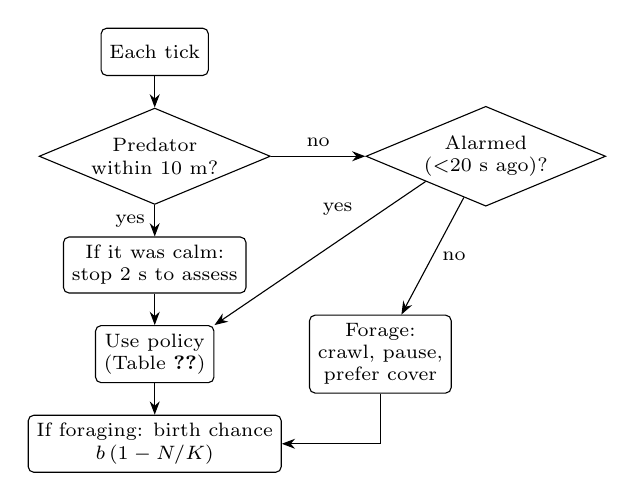
\begin{tikzpicture}[
  node distance=4mm and 6mm, font=\scriptsize, >=Stealth,
  box/.style={draw, rounded corners=2pt, align=center, minimum height=6mm, inner sep=3pt},
  dec/.style={draw, diamond, aspect=2.4, align=center, inner sep=1pt}]
\node[box] (start) {Each tick};
\node[dec, below=of start] (see) {Predator\\within 10 m?};
\node[dec, right=12mm of see] (alarm) {Alarmed\\($<$20 s ago)?};
\node[box, below=of see] (assess) {If it was calm:\\ stop 2 s to assess};
\node[box, below=of assess] (policy) {Use policy\\(Table~\ref{tab:policies})};
\node[box, right=12mm of policy] (forage) {Forage:\\crawl, pause,\\prefer cover};
\node[box, below=of policy] (breed) {If foraging: birth chance\\$b\,(1 - N/K)$};
\draw[->] (start) -- (see);
\draw[->] (see) -- node[left] {yes} (assess);
\draw[->] (see) -- node[above] {no} (alarm);
\draw[->] (alarm) -- node[right] {no} (forage);
\draw[->] (alarm.south west) -- node[above left, pos=0.3] {yes} (policy.north east);
\draw[->] (assess) -- (policy);
\draw[->] (policy) -- (breed);
\draw[->] (forage) |- (breed);
\end{tikzpicture}
\caption{What one octopus does in one tick. ``Alarmed'' means it saw a predator (or, with the social alarm on, a jetting neighbour) in the last 20~s. $b$ is the birth chance, $N$ the number of octopuses and $K$ the carrying capacity.}
\label{fig:flow}
\end{figure}

\paragraph{Detection.}
A predator sees an octopus on a patch with cover $c$ if they are at most
\begin{equation}
R = R_0 \,(1 - \kappa c)\,(1 - \gamma c)^{h}\,\mu^{m}
\label{eq:detect}
\end{equation}
apart.
Here $R_0 = 10$~m, $\kappa = 0.8$ is the effect of cover, $\gamma = 0.85$ is the strength of camouflage, $h = 1$ if the octopus is hiding, $\mu = 1.5$ is the effect of motion, and $m = 1$ if the octopus moved this tick.
So cover makes every octopus harder to see \cite{scharf2006}, camouflage only helps on cover \cite{hanlon2009}, and moving makes an octopus easier to see \cite{merilaita2017}.

\paragraph{Reproduction.}
Each tick, a foraging octopus gives birth with probability $b\,(1 - N/K)$, with $b = 0.005$ and $K = 250$, similar to Wolf Sheep Predation \cite{wilensky1997}.
Alarmed octopuses do not breed, so being careful has a cost \cite{mather1991}.
A newborn appears on a random patch, because real young octopuses drift away as larvae, and it gets its parent's policy.

\paragraph{Implementation.}
We wrote the model in NetLogo 7.0.4 \cite{wilensky1999}, split over ten source files.
Each tick, all octopuses act in random order, then all predators act, and then the population is recorded.
A run ends after 2000 ticks or when no octopus is left.
The Interface (Fig.~\ref{fig:interface}) has 13 controls, and all other constants are set in one procedure.
We also wrote a self test with 17 checks, for example that the cover mean hits its target, that jetting stops after 5~s, and that the same seed gives the same run.
Code and data are at \url{https://github.com/SkipsSkips/DMAS-15}.

\begin{figure}[tbp]
\centering
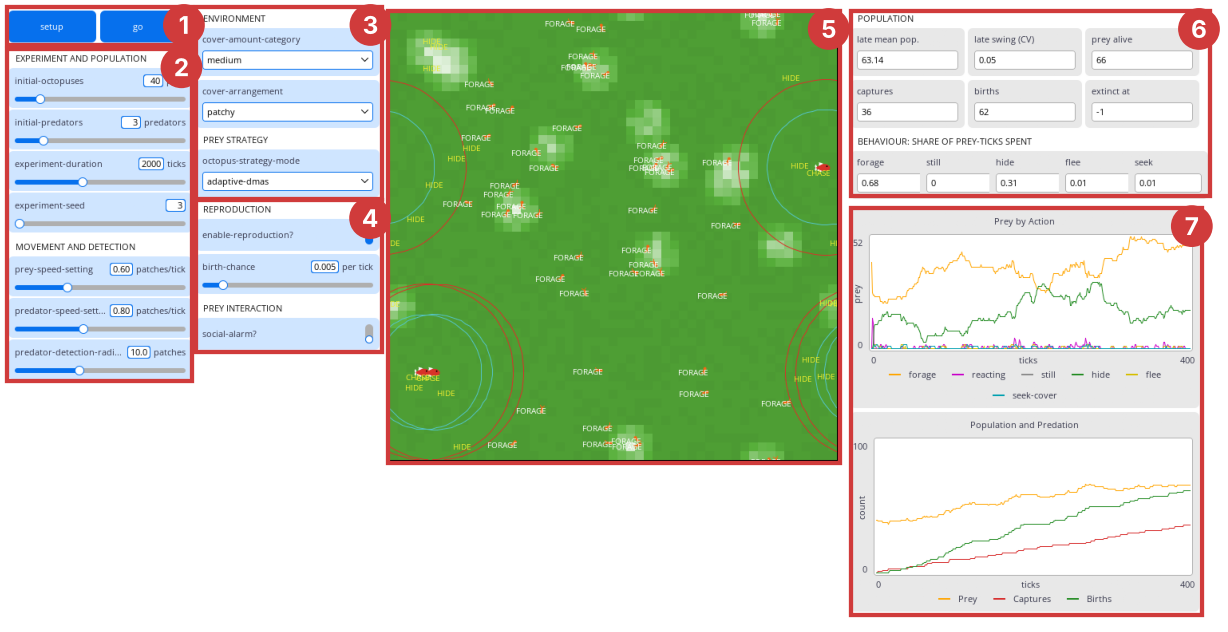
\includegraphics[width=\textwidth]{interface_annotated.png}
\caption{The Interface after 400 ticks (adaptive policy, patchy medium cover, seed 3). (1) Setup and go. (2) Population, run length, seed, speeds and detection radius. (3) Cover amount, arrangement and policy. (4) Reproduction and social alarm. (5) The world. Green shows cover, predators have a red ring (detection radius on sand) and a blue ring (radius on their current patch), and labels show what each agent is doing. (6) Monitors. (7) Live plots.}
\label{fig:interface}
\end{figure}

\subsection{Parameters}
Table~\ref{tab:params} lists the main parameters.
Where possible we took values from octopus and fish studies (``measured'').
Some values fit the biology but were not measured in this exact form (``plausible'').
The rest are our own modelling choices, or were tuned so that the model behaves sensibly (``calibration'').
The file \texttt{docs/PARAMETERS.md} in the repository explains every value.

\begin{table}[tbp]
\caption{Main parameters. M = measured, P = plausible, C = our choice, Cal = calibration.}
\label{tab:params}
\centering\scriptsize
\begin{tabular}{lrll}
\toprule
Parameter & Value & Unit & Source \\
\midrule
Initial octopuses / predators & 40 / 3 & - & P / C \\
Run length & 2000 & s (33 min) & C \\
Jet speed & 0.6 & m/s & M \cite{huffard2006} \\
Crawl speed & 0.09 & m/s & M \cite{huffard2006} \\
Pause share while foraging & 0.25 & - & M \cite{leite2009} \\
Home range radius & 10 & m & M \cite{papadopoulo2024} \\
Maximum jet time & 5 & s & M \cite{wells1987} \\
Jet recovery & 0.1 & s per s & C \\
Octopus notices predator within & 10 & m & P \\
Assessment time & 2 & s & C \\
Calm-down time & 20 & s & C \\
Predator chase / search speed & 0.8 / 0.4 & m/s & P \\
Base detection radius $R_0$ & 10 & m & P \\
Cover effect $\kappa$ & 0.8 & - & C \\
Camouflage $\gamma$ & 0.85 & - & C \\
Motion effect $\mu$ & 1.5 & - & C \\
Predator eating (handling) time & 20 & s & Cal \\
Birth chance $b$ & 0.005 & per s & Cal \\
Carrying capacity $K$ & 250 & octopuses & Cal \\
Alarm radius & 5 & m & C \\
\bottomrule
\end{tabular}
\end{table}

\subsection{Experiments and analysis}
We ran three experiments (Table~\ref{tab:design}).
Within one environment, a seed gives every policy the same world and the same starting positions, so we could compare policies in pairs.
For the mixed policy only the world is the same, because assigning policies uses extra random numbers.
Our main outcome is the late mean population, which is the average number of octopuses in the second half of the run (ticks 1000 to 2000). Runs that went extinct count as 0 after the extinction.
We also recorded extinctions, the coefficient of variation (CV) of the late population, births, captures and the time spent foraging.

\begin{table}[tbp]
\caption{Experiments. All runs last 2000 ticks (or until extinction) and start with 40 octopuses and 3 predators.}
\label{tab:design}
\centering\scriptsize
\begin{tabularx}{\textwidth}{lXlr}
\toprule
Experiment & What we varied & Seeds & Runs \\
\midrule
Environment & policy (6) $\times$ cover (low, medium, high) $\times$ arrangement (uniform, patchy), alarm off & 1-20 & 720 \\
Social alarm & policy (6) $\times$ cover (3) $\times$ alarm (off, on), patchy world & 1-20 & 720 \\
Sensitivity & 12 settings (the default, camouflage multiplier 0.05 and 0.3, motion multiplier 1.0 and 2.0, calm-down time 10 and 40~s, handling time 10 and 30~s, alarm radius 2.5, 5 and 10~m with the alarm on) $\times$ 2 environments (uniform low, patchy medium) $\times$ policy (6) & 1-10 & 1440 \\
\bottomrule
\end{tabularx}
\end{table}

We analysed the data in Python.
Many runs end close to zero, so the results are not normally distributed (a Shapiro-Wilk test rejected normality in 17 of 36 groups).
That is why we used rank-based tests, which do not assume a normal distribution.
To compare the six policies within one environment we used a Friedman test, and then a paired Wilcoxon test for every pair of policies (15 pairs).
As effect size we report the rank-biserial correlation $r$, which goes from $-1$ to $1$.
To compare uniform and patchy worlds we used Mann-Whitney tests, with Cliff's $\delta$ as effect size.
For extinctions we used Kaplan-Meier curves and log-rank tests, and for the alarm we again used paired Wilcoxon tests.
Because we ran many tests, we corrected the $p$-values with the Holm method \cite{holm1979}.
The biggest group of tests has 90 tests (15 pairs in 6 environments).
The 95\% confidence intervals (CI) come from bootstrapping with 10,000 resamples and are not corrected.

% ===================================================================
\section{Results}

\subsection{RQ1: Which policy gives the largest population?}
Fig.~\ref{fig:ts} shows the population over time and Table~\ref{tab:sweep} the late mean population.
At high cover all policies except still grew at about the same rate.
At low cover populations stayed small and often died out.
The policy had a significant effect in all six environments (Friedman tests, Table~\ref{tab:friedman}).

\begin{figure}[tbp]
\centering
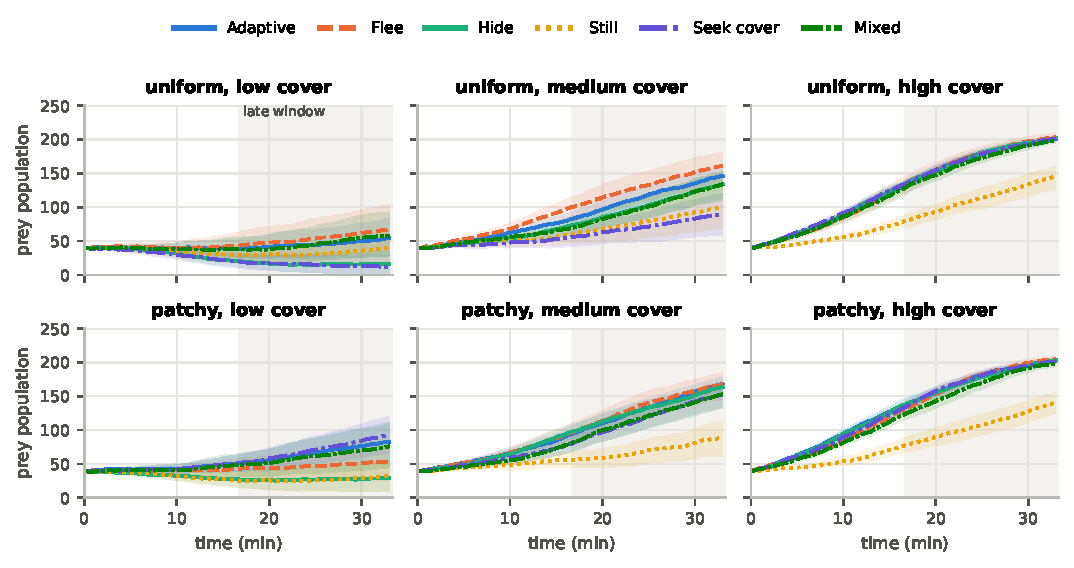
\includegraphics[width=\textwidth]{fig_timeseries.pdf}
\caption{Population over time, mean of 20 runs per line with 95\% bootstrap CI. Extinct runs count as 0. The grey band is the second half of the run, which we use for the late mean population.}
\label{fig:ts}
\end{figure}

\begin{table}[tbp]
\caption{Late mean population, mean (SD) over 20 seeds. Bold: highest mean in the environment. Superscript: runs (out of 20) that went extinct.}
\label{tab:sweep}
\centering\scriptsize
\resizebox{\textwidth}{!}{\begin{tabular}{lrrrrrr}
\toprule
 & \multicolumn{3}{c}{Uniform} & \multicolumn{3}{c}{Patchy} \\
\cmidrule(lr){2-4}\cmidrule(lr){5-7}
Policy & Low & Medium & High & Low & Medium & High \\
\midrule
adaptive & 45.5 (50.2)$^{9}$ & 116.6 (32.8) & 175.8 (12.0) & 66.6 (50.3)$^{1}$ & 133.1 (30.4) & 176.9 (12.5) \\
flee & \textbf{54.4 (66.3)}$^{12}$ & \textbf{132.8 (48.2)}$^{1}$ & \textbf{176.4 (22.7)} & 47.4 (49.9)$^{8}$ & \textbf{136.7 (41.9)} & \textbf{177.0 (14.0)} \\
hide & 16.2 (32.0)$^{17}$ & 103.4 (37.6) & 174.8 (11.7) & 27.1 (40.4)$^{11}$ & 131.9 (24.4) & 175.5 (14.2) \\
still & 32.6 (42.6)$^{12}$ & 79.9 (54.5)$^{3}$ & 113.7 (32.3) & 26.9 (40.3)$^{14}$ & 70.1 (42.8)$^{1}$ & 108.6 (35.1) \\
seek-cover & 15.0 (30.9)$^{17}$ & 72.5 (53.0)$^{2}$ & 174.7 (10.0) & \textbf{71.0 (46.4)} & 119.1 (34.5) & 176.7 (11.6) \\
mixed & 46.2 (60.2)$^{12}$ & 102.0 (38.7) & 170.0 (16.2) & 61.4 (60.3)$^{7}$ & 120.1 (40.6) & 167.5 (18.5) \\
\bottomrule
\end{tabular}
}
\end{table}

\begin{table}[tbp]
\caption{Friedman test over the six policies per environment ($n = 20$), and the paired difference flee minus hide. The CI is not corrected for multiple tests.}
\label{tab:friedman}
\centering\scriptsize
\resizebox{\textwidth}{!}{\begin{tabular}{llrrrrr}
\toprule
Arrangement & Cover & $\chi^2_{\mathrm{F}}(5)$ & $p_\mathrm{Holm}$ & Kendall's $W$ & Flee $-$ hide [95\% CI] & $r$ \\
\midrule
uniform & low & 13.4 & 0.020 & 0.13 & +38.2 [+16.6, +61.5] & +0.62 \\
uniform & medium & 26.5 & $<$0.001 & 0.26 & +29.4 [+8.5, +51.3] & +0.71 \\
uniform & high & 42.6 & $<$0.001 & 0.43 & +1.6 [-8.5, +10.3] & +0.24 \\
patchy & low & 27.9 & $<$0.001 & 0.28 & +20.3 [-3.6, +44.9] & +0.39 \\
patchy & medium & 27.3 & $<$0.001 & 0.27 & +4.8 [-14.0, +21.5] & +0.35 \\
patchy & high & 43.0 & $<$0.001 & 0.43 & +1.5 [-6.1, +9.0] & +0.10 \\
\bottomrule
\end{tabular}
}
\end{table}

\paragraph{Hide or flee (H1).}
Fleeing gave more octopuses than hiding in uniform low cover ($+38.2$, CI $[+16.6, +61.5]$) and uniform medium cover ($+29.4$, CI $[+8.5, +51.3]$).
However, neither difference was significant after the Holm correction over 90 tests.
At high cover the two policies were almost equal ($+1.6$ uniform, $+1.5$ patchy).
Hiding never did better than fleeing.

\paragraph{The adaptive policy (H2).}
Adaptive never had the highest mean.
Flee was best in five environments and seek-cover in patchy low cover.
Still, adaptive was never significantly worse than any policy except still, and over all environments it was almost equal to flee (119.1 against 120.8, Table~\ref{tab:pooled}).
In total, 15 of the 90 pairwise tests were significant after correction.
Fourteen of them were still losing to another policy at medium or high cover. The last one was flee beating seek-cover in uniform medium cover.

\paragraph{Cover arrangement (H3).}
The arrangement mattered most for seek-cover.
At low cover it reached 71.0 in patchy worlds against 15.0 in uniform worlds (Cliff's $\delta = 0.78$, $p_\mathrm{Holm} < 0.001$).
No other policy and cover level differed significantly by arrangement.

\paragraph{Mixed populations.}
In the mixed runs, the policies that did well on their own also spread (Table~\ref{tab:mixed}).
Flee took over in uniform low and medium cover (shares 0.87 and 0.76), seek-cover and flee shared patchy low cover, and still almost disappeared everywhere.

\subsection{RQ2: Population stability}
Extinctions happened almost only at low cover, and never at high cover (Fig.~\ref{fig:ext}).
At low cover, 10 of 40 adaptive populations died out, against 20 for flee, 28 for hide and 26 for still (Table~\ref{tab:pooled}).
Log-rank tests against adaptive were significant for hide ($\chi^2 = 15.5$, $p_\mathrm{Holm} < 0.001$) and still ($\chi^2 = 13.7$, $p_\mathrm{Holm} < 0.001$).
For flee the test gave $p = 0.020$ before and $0.061$ after correction.
In runs that survived, fluctuations were small (late CV 0.16 to 0.19 on average).

\begin{figure}[tbp]
\centering
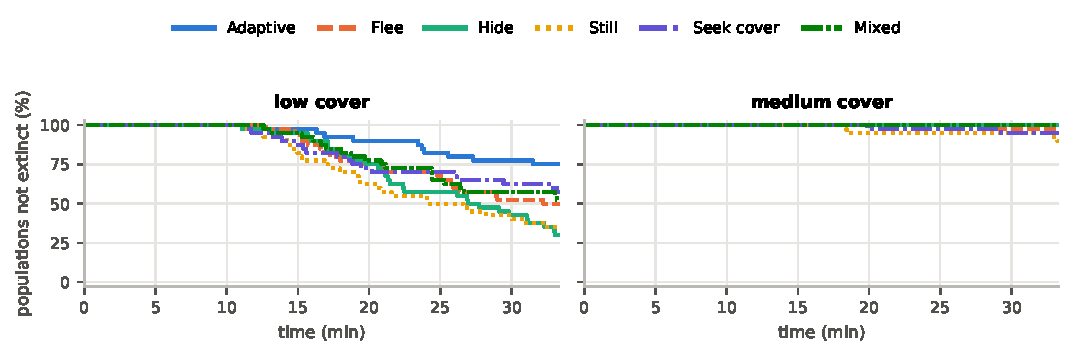
\includegraphics[width=\textwidth]{fig_extinction.pdf}
\caption{Kaplan-Meier curves: share of populations not yet extinct, uniform and patchy worlds together ($n = 40$ per line). No high-cover run went extinct.}
\label{fig:ext}
\end{figure}

\begin{table}[tbp]
\caption{All six environments together ($n = 120$ runs per policy). CV: mean late coefficient of variation of the runs that survived.}
\label{tab:pooled}
\centering\scriptsize
\begin{tabular}{lrrrr}
\toprule
Policy & Late mean pop. [95\% CI] & Extinct runs & Extinct, low cover & CV (surviving) \\
\midrule
adaptive & 119.1 [107.9, 129.7] & 10/120 & 10/40 & 0.169 \\
flee & 120.8 [108.2, 132.9] & 21/120 & 20/40 & 0.159 \\
hide & 104.8 [92.3, 116.7] & 28/120 & 28/40 & 0.160 \\
still & 72.0 [62.4, 81.4] & 30/120 & 26/40 & 0.194 \\
seek-cover & 104.8 [92.3, 117.0] & 19/120 & 17/40 & 0.175 \\
mixed & 111.2 [99.8, 122.4] & 19/120 & 19/40 & 0.184 \\
\bottomrule
\end{tabular}

\end{table}

\subsection{RQ3: Social alarm}
With the alarm on, an octopus that sees a neighbour jet within 5~m becomes alarmed too.
This lowered the flee population from 120.4 to 61.8 (difference $-58.6$, CI $[-71.1, -46.0]$, $p_\mathrm{Holm} < 0.001$, see Fig.~\ref{fig:alarm} and Table~\ref{tab:alarm}).
Mixed populations went down by 30.5.
Hide and still did not change at all, because these octopuses never jet, so they never set off an alarm.
For adaptive the change was small and not significant ($+4.6$).

The alarm did save some flee octopuses, since captures went down from 179 to 136 per run.
But births went down much more, from 282 to 173, and the time spent foraging dropped from 66\% to 52\%.

\begin{figure}[tbp]
\centering
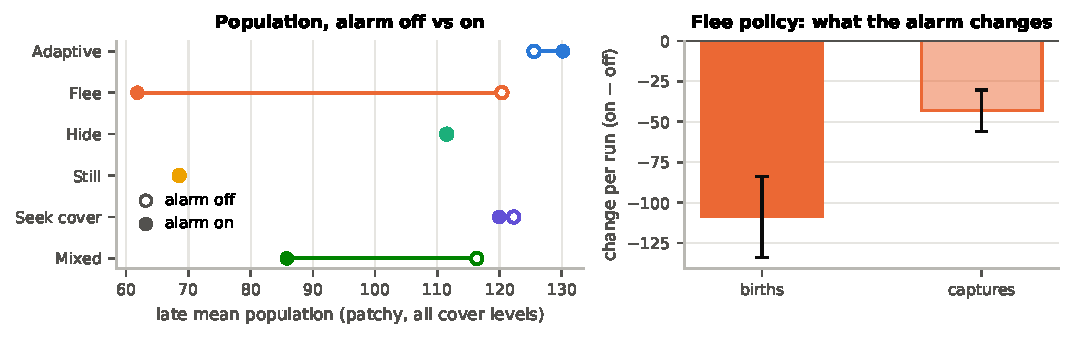
\includegraphics[width=\textwidth]{fig_social_alarm.pdf}
\caption{Social alarm, patchy world, all cover levels together ($n = 60$ pairs per policy). Left: late mean population with the alarm off (open) and on (filled). Right: change in births and captures per run for flee (mean and 95\% bootstrap CI).}
\label{fig:alarm}
\end{figure}

\begin{table}[tbp]
\caption{Social alarm off and on, paired by seed (patchy world, three cover levels, $n = 60$ pairs per policy). $p$-values are Holm-corrected over the six policies.}
\label{tab:alarm}
\centering\scriptsize
\resizebox{\textwidth}{!}{\begin{tabular}{lrrrrrrr}
\toprule
Policy & Off & On & On $-$ off [95\% CI] & $r$ & $p_\mathrm{Holm}$ & Births & Captures \\
\midrule
adaptive & 125.5 & 130.2 & +4.6 [-5.0, +14.5] & +0.17 & 1.000 & 297$\to$308 & 184$\to$189 \\
flee & 120.4 & 61.8 & -58.6 [-71.1, -46.0] & -0.91 & $<$0.001 & 282$\to$173 & 179$\to$136 \\
hide & 111.5 & 111.5 & 0 (identical runs) & - & - & 271$\to$271 & 179$\to$179 \\
still & 68.5 & 68.5 & 0 (identical runs) & - & - & 241$\to$241 & 193$\to$193 \\
seek-cover & 122.3 & 119.9 & -2.4 [-7.8, +2.2] & -0.01 & 1.000 & 300$\to$291 & 190$\to$187 \\
mixed & 116.3 & 85.8 & -30.5 [-41.8, -19.6] & -0.68 & $<$0.001 & 288$\to$237 & 185$\to$171 \\
\bottomrule
\end{tabular}
}
\end{table}

\subsection{Sensitivity}
Fig.~\ref{fig:sens} shows what happened when we changed one of our own choices at a time (10 seeds per point).
The predator's handling time mattered most. With 10~s almost every population died out, and with 30~s all policies reached high populations.
Stronger camouflage made hide the best policy in patchy medium cover.
A shorter calm-down time favoured flee, and a longer one lowered every population.
A larger alarm radius removed almost all flee octopuses.
Over the nine settings without the alarm, flee was still the best in uniform low cover six times, and adaptive was the best in patchy medium cover six times.

\begin{figure}[tbp]
\centering
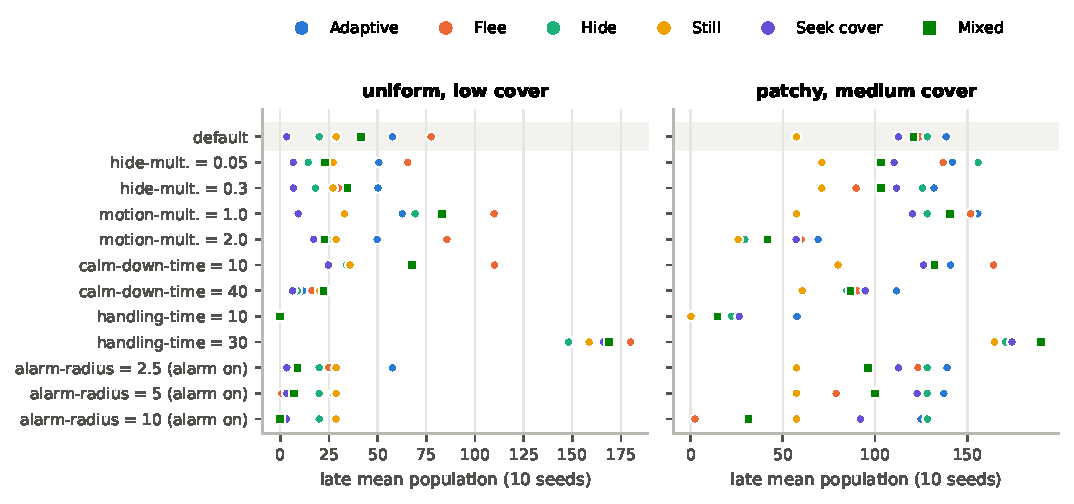
\includegraphics[width=\textwidth]{fig_sensitivity.pdf}
\caption{Sensitivity runs: late mean population per policy (mean of 10 seeds) for each setting. ``mult.'' is the camouflage or motion multiplier. The default setting is shaded. The alarm-radius rows have the alarm on.}
\label{fig:sens}
\end{figure}

% ===================================================================
\section{Discussion}

\paragraph{RQ1.}
H1 is only half supported.
Fleeing was better than hiding when cover was low and uniform, as escape theory predicts \cite{broom2005}.
But we expected hiding to win at high cover, and it only tied.
We think this is because a fleeing octopus in our model hides as soon as its jet runs out, and in dense cover this ``jet, then hide'' works just as well as hiding straight away.
H2 is not supported, since adaptive was never the best on average, although it was never significantly worse than the best policy.
H3 is supported. Seek-cover only works when there is dense cover nearby, which at low cover only the patchy world has.

\paragraph{RQ2.}
H4 is supported.
Adaptive had the fewest extinctions, clearly fewer than hide and still.
Each fixed policy fails in some situations. Hiding fails on open sand, and fleeing fails when the predator is close and the jet is used up.
Adaptive switches between the two, so it rarely has a run of bad luck that wipes out the population.
It gives up a little of its average size for a lower risk of collapse, and for a real population that may be the better deal.

\paragraph{RQ3.}
H5 is rejected, which surprised us.
The alarm made populations of jetting octopuses smaller, because alarmed neighbours stopped feeding and therefore stopped breeding.
The captures they avoided did not make up for the lost births.
This fits escape theory, which counts lost feeding time as a cost of reacting \cite{ydenberg1986}: here, too much vigilance cost more than it saved.
The alarm also spreads. One jet alarms the neighbours, and they jet and alarm their own neighbours.
With a 10~m alarm radius, fleeing octopuses in patchy medium cover foraged only 39\% of the time and the population almost disappeared.
Adaptive octopuses only jet when they are chased, so they rarely start an alarm, and the alarm did not hurt them.

\paragraph{Limitations.}
The biggest one is that we sped up time.
Real octopuses breed once in their life, but ours can give birth every second, so that population effects show up within a 33-minute run.
Because of this, predators also have to kill far too often. They catch about 109 octopuses per predator per hour, while a grouper hunting alone was seen to catch about 0.04 prey per hour \cite{bshary2006}.
So our numbers should only be compared with each other, not with real populations.
Several parameters are our own choices, and the sensitivity runs show that the best policy can change when they change, especially the handling time.
We only have visual predators. Moray eels, which search crevices \cite{bshary2006}, would give hiding a real cost.
Offspring simply copy their parent's policy, which is not how octopus genetics works.
Finally, the runs are short. At medium and high cover the population is still growing when the run ends, so we measure it on the way up and not at its final size.
With only 20 seeds and 90 corrected tests, some differences of 20 to 40 octopuses were also not significant.

\paragraph{Future work.}
The most useful next step would be a second predator that searches crevices.
It would also help to run longer simulations with more seeds, and to let octopuses learn their policy during their life instead of inheriting it.

% ===================================================================
\section{Conclusion}
We built an agent-based model of octopuses that forage, notice predators nearby and choose how to react.
No single policy was best everywhere.
Fleeing gave the largest populations when cover was scarce and uniform, and with plenty of cover hiding and fleeing were equal.
Moving to cover only worked when dense cover was close.
The adaptive ``hide until chased'' policy was never the best on average, but it died out least often.
A social alarm made things worse, because alarmed octopuses stopped feeding.
Since many parameters are our own choices, these results show possible mechanisms, not measured octopus behaviour.

% ===================================================================
\section{Division of Labour}
\begin{itemize}
\item Alex Pavel: model versions 1 to 3 (foraging, jet limit, adaptive policy, social alarm), the experiments and the statistical analysis.
\item Nazariy Pavlishak: the code structure of version 3, the population model, the Interface and the self test.
\item Alexia Zaharie: the report and the biology background, including checking the references.
\item Andrei Razaroiu: the presentation, the sensitivity analysis and the limitations.
\end{itemize}

\bibliographystyle{splncs04}
\bibliography{references}

% ===================================================================
\appendix

\section{Reproducing the Results}
\label{app:repro}
\begin{enumerate}
\item Install NetLogo 7.0.4 and Python 3 with NumPy, SciPy, pandas and Matplotlib.
\item Clone the repository at \url{https://github.com/SkipsSkips/DMAS-15}.
\item Open \texttt{octoplus-v3.nlogox} and run \texttt{run-self-test} in the Command Center. It should print \texttt{RESULT: PASS}.
\item Run the two main experiments headless (about 6 minutes each on two cores):
\begin{verbatim}
java -Xmx4g -cp "NetLogo 7.0.4/lib/app/*" \
  org.nlogo.headless.Main \
  --model octoplus-v3.nlogox \
  --experiment environment-sweep \
  --table results/v3/environment-sweep.csv \
  --threads 2
\end{verbatim}
Then do the same with experiment \texttt{social-alarm}.
\item Run the sensitivity sweep, which takes about 40 minutes:\\ \texttt{experiments/run\_sensitivity.sh}
\item Make all figures and tables with the two analysis scripts:\\ \texttt{analysis/v3\_analysis.py} and \texttt{analysis/v3\_tables.py}
\end{enumerate}
The seed is set with a slider, so the same seed, settings and NetLogo version always give the same result.

\section{Compact ODD Description}
\label{app:odd}
\begin{table}[H]
\caption{ODD summary \cite{grimm2020}. More details are in Section~2 and \texttt{docs/PARAMETERS.md}.}
\label{tab:odd}
\centering\scriptsize
\begin{tabularx}{\textwidth}{lX}
\toprule
Element & Description \\
\midrule
Purpose & Find out which anti-predator policy gives the largest and most stable octopus population, depending on the amount and arrangement of cover, and whether a social alarm helps. \\
Entities & Octopuses (policy, action, home patch, jet time, alarm timer), predators (speed, detection radius, target, handling timer) and patches (cover 0 to 1). \\
Scales & 1 patch = 1 m, 1 tick = 1 s, a $51 \times 51$ m wrapping world, and 2000 ticks (33 min) per run. \\
Process overview & Each tick, the octopuses act first in random order (look, assess, use policy or forage, maybe breed). Then the predators act (eat, chase or wander, catch). Then the population is recorded. \\
Design concepts & Emergence: population size, extinction and the policy mix. Sensing: local only (10 m for predators, 5 m for jetting neighbours). Adaptation: the adaptive policy changes its action with the situation. Interaction: predation and the optional alarm. Stochasticity: world, start positions, foraging, births, order of actions. \\
Initialisation & Make the cover and rescale it to the target mean. Place 40 octopuses and 3 predators at random, all calm with full jet time. \\
Submodels & Detection (Eq.~\ref{eq:detect}), foraging walk that prefers cover, jet limit and recovery, adaptive rule (Table~\ref{tab:policies}) and birth chance $b(1-N/K)$. \\
\bottomrule
\end{tabularx}
\end{table}

\section{Additional Material}
\label{app:extra}
\begin{table}[H]
\caption{Policy shares at the end of the mixed runs that did not go extinct. Every run started with about equal shares. Bold: largest share.}
\label{tab:mixed}
\centering\scriptsize
\begin{tabular}{llrrrrr}
\toprule
Arrangement & Cover & Surviving runs & still & hide & flee & seek-cover \\
\midrule
uniform & low & 8/20 & 0.02 & 0.09 & \textbf{0.87} & 0.02 \\
uniform & medium & 20/20 & 0.03 & 0.19 & \textbf{0.76} & 0.03 \\
uniform & high & 20/20 & 0.04 & 0.30 & 0.31 & \textbf{0.35} \\
patchy & low & 13/20 & 0.02 & 0.06 & 0.44 & \textbf{0.48} \\
patchy & medium & 20/20 & 0.05 & 0.21 & \textbf{0.51} & 0.24 \\
patchy & high & 20/20 & 0.04 & \textbf{0.39} & 0.27 & 0.30 \\
\bottomrule
\end{tabular}

\end{table}
\begin{figure}[H]
\centering
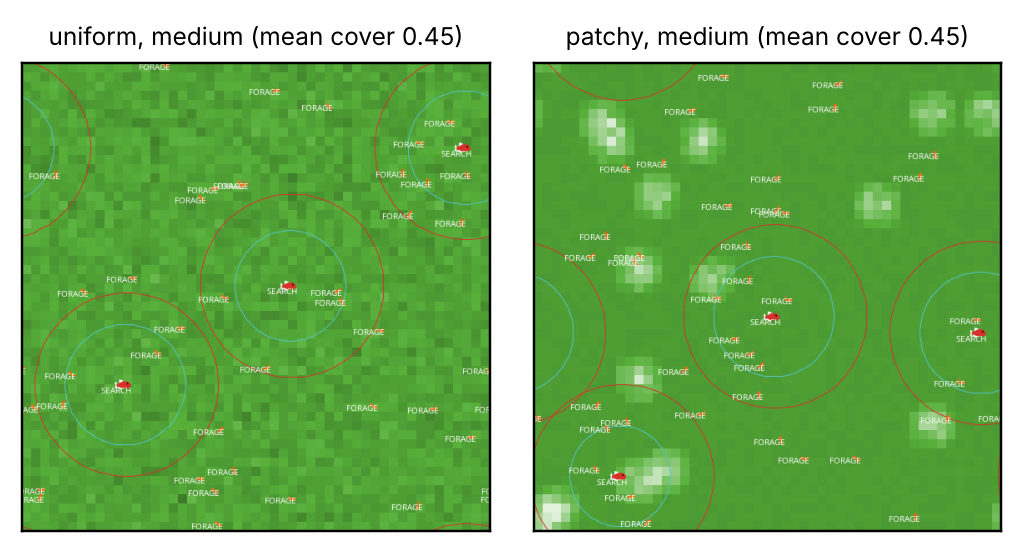
\includegraphics[width=0.7\textwidth]{environments.png}
\caption{Two worlds with the same mean cover (0.45), uniform and patchy, seed 3. Lighter green is denser cover.}
\label{fig:env}
\end{figure}

\paragraph{How the model changed.}
Our first version used one strategy for the whole population, had no seed control, and its patchy worlds had 72\% less cover than the uniform ones.
In version 2 we added seeds, cover rescaling and reproduction, but we later found that its fleeing octopuses could sense predators anywhere in the world.
Version 3, used in this report, has local sensing only, foraging, the jet limit, handling time and the social alarm.

\end{document}
